\documentclass[12pt, a4paper]{report}
\usepackage{graphicx, array, amsthm, amssymb, amsmath, algorithm, algpseudocode, float, xcolor, thmtools, thmbox, exercise}
\usepackage[english]{babel}

\makeatletter
\renewcommand\thmbox@headstyle[2]{\bfseries #1}
\makeatother
\newtheorem[style=M,bodystyle=\normalfont]{theorem}{Theorem}
\newtheorem[style=M,bodystyle=\normalfont]{corollary}{Corollary}
\newtheorem[style=M,bodystyle=\normalfont]{lemma}{Lemma}
\newtheorem[style=M,bodystyle=\normalfont]{definition}{Definition}


\title{Data Bases II \\ \textit{Exercises}}
\author{Christian Rossi}
\date{Academic Year 2023-2024}

\begin{document}

\maketitle

\newpage

\begin{abstract}
    The course aims to prepare software designers on the effective development of database applications. First, the course presents the fundamental features of current database 
    architectures, with a specific emphasis on the concept of transaction and its realization in centralized and distributed systems. Then, the course illustrates the main directions 
    in the evolution of database systems, presenting approaches that go beyond the relational model, like active databases, object systems and XML data management solutions.
\end{abstract}

\newpage

\tableofcontents

\newpage

\chapter{Exerise session I}
    \begin{Exercise}[label=1]
        Can the following schedules produce anomalies? $c_i$ and $a_i$ indicate the transactional decision (commit/abort). 
        \begin{enumerate}
            \item $r_1(x) w_1(x) r_2(x) w_2(y)\:a_1\:c_2$
            \item $r_1(x) w_1(x) r_2(y) w_2(y)\:a_1\:c_2$
            \item $r_1(x) r_2(x) r_2(y) w_2(y) r_1(z)\:a_1\:c_2$
            \item $r_1(x) r_2(x) w_2(x) w_1(x)\:c_1\:c_2$
            \item $r_1(x) r_2(x) w_2(x) r_1(y)\:c_1\:c_2$
            \item $r_1(x) w_1(x) r_2(x) w_2(x)\:c_1\:c_2$
        \end{enumerate}
    \end{Exercise}
    \begin{Answer}[ref=1]
        \begin{enumerate}
            \item We have a serial execution, but with the abort of the first transaction. Since the second transaction reads the modified value of $x$ before the abort, we have a
                dirty read. 
            \item We have a serial execution and the two transactions require different resources, so there are no anomalies.
            \item There are no anomalies because the last operation of the first transaction works on a different resource. 
            \item Both transactions first reads in sequence the resource $x$ and then updates it without considering the updated value, so we have a lost update. 
            \item There are no anomalies because the last operation of the first transaction works on a different resource. 
            \item We have a serial execution, so the schedule is correct. 
        \end{enumerate}
    \end{Answer}

    \newpage
    
    \begin{Exercise}[label=2]
        The following schedule may produce 2 anomalies: a lost update and a phantom update. Identify them. 
        \[r_1(x) r_2(x) r_3(x) w_1(x) r_4(y) w_2(x) r_4(x) w_4(y) r_3(y)w_4(x) r_5(y) w_6(y) w_5(y) w_7(y)\]
    \end{Exercise}
    \begin{Answer}[ref=2]
        We can write the schedule in the following way: 
    \begin{table}[H]
        \centering
        \resizebox{\textwidth}{!}{%
        \begin{tabular}{cccccccccccccc}
        $r_1(x)$           &           &                    & $w_1(x)$           & \textbf{} & \textbf{} & \textbf{} & \textbf{} & \textbf{} & \textbf{} & \textbf{} & \textbf{} & \textbf{} & \textbf{} \\
                        & $r_2(x)$  & \textit{\textbf{}} & \textit{\textbf{}} & \textbf{} & $w_2(x)$  & \textbf{} & \textbf{} & \textbf{} & \textbf{} & \textbf{} & \textbf{} & \textbf{} & \textbf{} \\
        \textit{\textbf{}} & \textbf{} & $r_3(x)$           & \textbf{}          & \textbf{} & \textbf{} & \textbf{} & \textbf{} & $r_3(y)$  & \textbf{} & \textbf{} & \textbf{} & \textbf{} & \textbf{} \\
        \textit{\textbf{}} & \textbf{} & \textbf{}          &                    & $r_4(y)$  & \textbf{} & $r_4(x)$  & $w_4(y)$  & \textbf{} & $w_4(x)$  & \textbf{} & \textbf{} & \textbf{} & \textbf{} \\
        \textit{\textbf{}} & \textbf{} & \textbf{}          & \textbf{}          & \textbf{} & \textbf{} & \textbf{} & \textbf{} & \textbf{} & \textbf{} & $r_5(y)$  & \textbf{} & $w_5(y)$  & \textbf{} \\
        \textbf{}          & \textbf{} & \textbf{}          & \textbf{}          & \textbf{} & \textbf{} & \textbf{} & \textbf{} & \textbf{} & \textbf{} & \textbf{} & $w_6(y)$  & \textbf{} & \textbf{} \\
        \textbf{}          & \textbf{} & \textbf{}          & \textbf{}          & \textbf{} & \textbf{} & \textbf{} & \textbf{} & \textbf{} & \textbf{} & \textbf{} & \textbf{} & \textbf{} & $w_7(y)$ 
        \end{tabular}%
        }
    \end{table}
        And we can see that there is a lost update with transactions $T_1$ and $T_2$ and a phantom update with $T_3$ and $T_4$. 
    \end{Answer}

    \newpage
    
    \begin{Exercise}[label=3]
        Classify the following schedule: 
        \[r_1(x) r_2(y) w_3(y) r_5(x) w_5(u) w_3(s)w_2(u) w_3(x) w_1(u) r_4(y) w_5(z) r_5(z)\]
    \end{Exercise}
    \begin{Answer}[ref=3]
        Since CSR contains VSR we check with the conflict graph. To do so we first divide the schedule based on the resources: 
        \begin{itemize}
            \item $x: r_1 \: r_5 \:w_3$
            \item $y: r_2 \: w_3 \:r_4$
            \item $z: w_5 \: r_5$
            \item $s: w_3$
            \item $u: w_5 \: w_2 \:w_1$
        \end{itemize}
        The nodes are $\{1,2,3,4,5\}$ and the arcs are found with the write-write or write-read relations found in the previous groups. So we have the following graph:
        \begin{figure}[H]
            \centering
            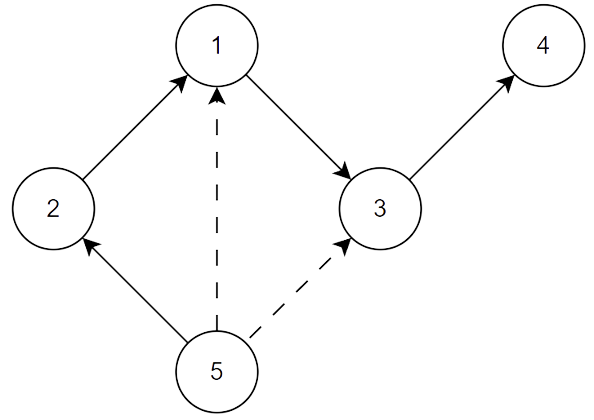
\includegraphics[width=0.5\linewidth]{images/conflictgraph.png}
        \end{figure}
        Some arcs can be omitted if the nodes are connected in another way (in this case we can remove arcs $\{\{5,1\},\{5,3\}\}$). 

        There are no cycles: the schedule is CSR (and also VSR). 
    \end{Answer}

    \newpage
    
    \begin{Exercise}[label=4]
        Classify the following schedule: 
        \[r_2(u) w_2(s) r_1(x) r_2(y) w_3(y) r_5(x) w_5(u) w_3(s)w_2(u) w_3(x) w_1(u) r_4(y) w_5(z) r_5(z)\]
    \end{Exercise}
    \begin{Answer}[ref=4]
        Since CSR contains VSR we check with the conflict graph. To do so we first divide the schedule based on the resources: 
        \begin{itemize}
            \item $x: r_1 \: r_5 \:w_3$
            \item $y: r_2 \: w_3 \:r_4$
            \item $z: w_5 \: r_5$
            \item $s: w_2 \: w_3$
            \item $u: r_2 \: w_5 \: w_2 \:w_1$
        \end{itemize}
        The nodes are $\{1,2,3,4,5\}$ and the arcs are found with the write-write or write-read relations found in the previous groups. So we have the following graph:
        \begin{figure}[H]
            \centering
            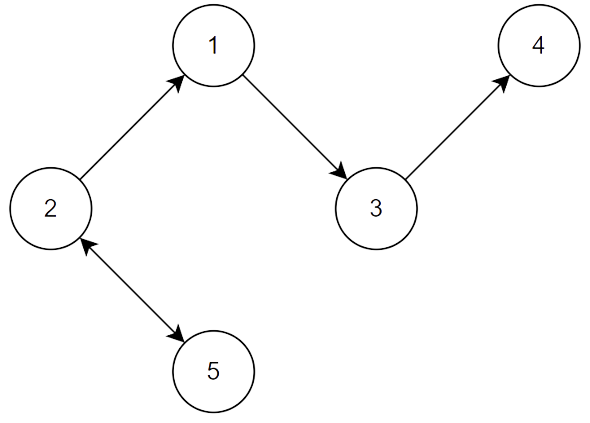
\includegraphics[width=0.5\linewidth]{images/conflictgraph1.png}
        \end{figure}
        It is possible to see that there is a cycle between two and five. The definition of VSR states that we need to have the same reads-from relations and final writes. So, we try to find a view-equivalent 
        schedule that is also CSR. One possible solution is simply to swap the two writes on the resource $u$ and that is sufficient to eliminate the cycle. So, the schedule: 
        \[r_2(u) w_2(s) r_1(x) r_2(y) w_3(y) r_5(x) w_5(u) w_2(u) w_3(s) w_3(x) w_1(u) r_4(y) w_5(z) r_5(z)\]
        is CSR and also VSR. 
    \end{Answer}

    \newpage
    
    \begin{Exercise}[label=5]
        Classify the following schedule: 
        \[r_1(x) r_2(y) w_3(y) r_5(x) w_5(u) w_3(s)w_2(u) w_3(x) w_1(u) r_4(y) w_5(z) r_5(z) r_2(u) w_2(s)\]
    \end{Exercise}
    \begin{Answer}[ref=5]
        Since CSR contains VSR we check with the conflict graph. To do so we first divide the schedule based on the resources: 
        \begin{itemize}
            \item $x: r_1 \: r_5 \: w_3$
            \item $y: r_2 \: w_3 \: r_4$
            \item $z: w_5 \: r_5$
            \item $s: w_3 \: w_2$
            \item $u: w_5 \: w_2 \: w_1 \: r_2$
        \end{itemize}
        The nodes are $\{1,2,3,4,5\}$ and the arcs are found with the write-write or write-read relations found in the previous groups. So we have the following graph:
        \begin{figure}[H]
            \centering
            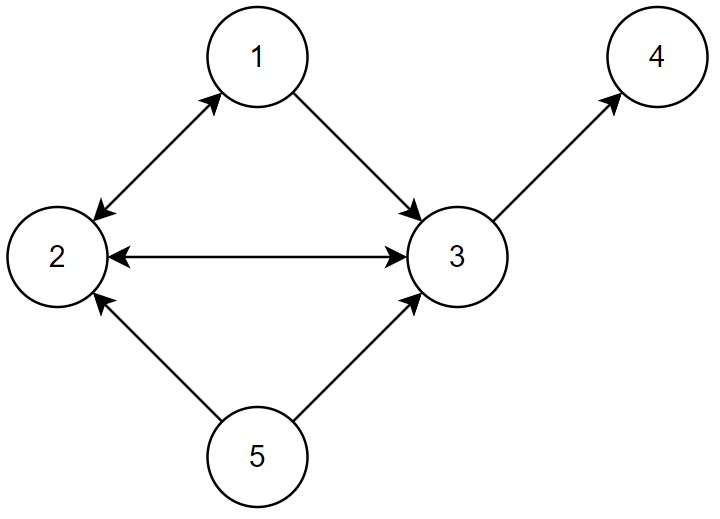
\includegraphics[width=0.5\linewidth]{images/conflictgraph2.png}
        \end{figure}
        In this case it is not possible to find a VSR schedule because it is impossible to do so without changing the final write on $s$. 
    \end{Answer}

    \newpage

    \begin{Exercise}[label=6]
        Classify the following schedule: 
        \[r_5(x) r_3(y) w_3(y) r_6(t) r_5(t) w_5(z) w_4(x) r_3(z) w_1(y) \dots\]
        \[\dots r_6(y) w_6(t) w_4(z) w_1(t) w_3(x) w_1(x) r_1(z) w_2(t) w_2(z)\]
    \end{Exercise}
    \begin{Answer}[ref=6]
        Since CSR contains VSR we check with the conflict graph. To do so we first divide the schedule based on the resources: 
        \begin{itemize}
            \item $t: \: r_6 \: r_5 \: w_6 \: w_1 \: w_2$
            \item $x: \: r_5 \: w_4 \: w_3 \: w_1$
            \item $y: \: r_3 \: w_3 \: w_1 \: r_6$
            \item $z: \: w_5 \: r_3 \: w_4 \: r_1 \: w_2$
        \end{itemize}
        The nodes are $\{1,2,3,4,5,6\}$ and the arcs are found with the write-write or write-read relations found in the previous groups. So we have the following graph:
        \begin{figure}[H]
            \centering
            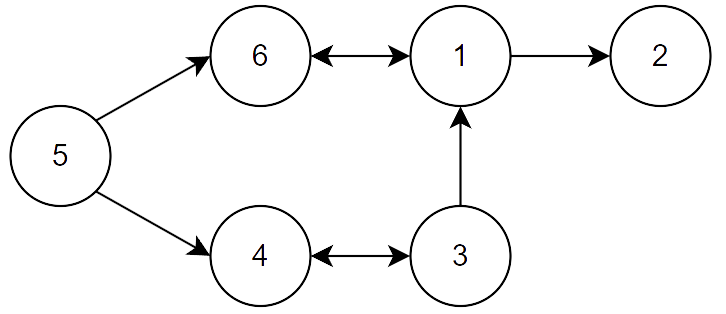
\includegraphics[width=0.5\linewidth]{images/conflictgraph3.png}
        \end{figure}
        We have two cycles. It is impossible to find a VSR schedule because only the conflict between four and three can be eliminated (the other one changes a read-write relation).
    \end{Answer}

    \newpage

\end{document}